\clearpage

\section{Optical Hybrid}

\begin{tcolorbox}	
	\begin{tabular}{p{2.75cm} p{0.2cm} p{10.5cm}} 	
		\textbf{Header File}   &:& optical\_hybrid.h \\
		\textbf{Source File}   &:& optical\_hybrid.cpp \\
	\end{tabular}
\end{tcolorbox}

This block simulates an optical hybrid. It accepts two input signals corresponding to the signal and to the local oscillator. It generates four output complex signals separated by $90^\circ$ in the complex plane. Figure ~\ref{opticalhybrid} shows a schematic representation of this block.

\begin{figure}[h]
	\centering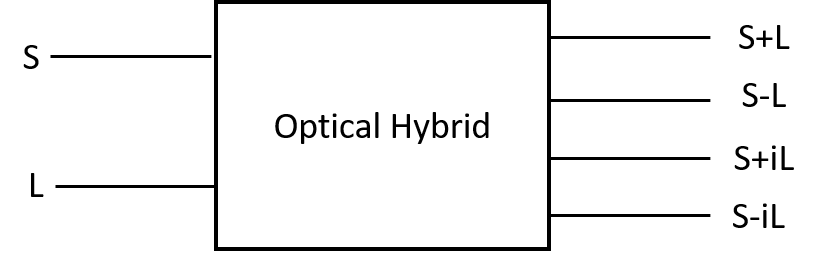
\includegraphics[width=0.6\textwidth]{./lib/optical_hybrid/figures/optical_hybrid_block_diagram.png}
	\caption{Schematic representation of an optical hybrid.}\label{opticalhybrid}
\end{figure}

\subsection*{Input Parameters}

\begin{table}[h]
	\centering
	\begin{tabular}{|c|c|c|c|ccp{60mm}}
		\cline{1-4}
		\textbf{Parameter} & \textbf{Type} & \textbf{Values} &   \textbf{Default}& \\ \cline{1-4}
		outputOpticalPower & double & any & $1e-3$ \\ \cline{1-4}
		outputOpticalWavelength & double & any & $1550e-9$ \\ \cline{1-4}
		outputOpticalFrequency & double & any & SPEED\_OF\_LIGHT / outputOpticalWavelength \\ \cline{1-4}
		powerFactor & double & $\leq 1$ & $0.5$ \\ \cline{1-4} 
	\end{tabular}
	\caption{Optical hybrid input parameters}
	\label{table:optical_hybrid_in_par}
\end{table}

%\begin{itemize}
%	\item outputOpticalPower\{ 1e-3 \} 
%	\item outputOpticalWavelength\{ 1550e-9 \}
%	\item outputOpticalFrequency\{ SPEED\_OF\_LIGHT / wavelength \}
%	\item powerFactor\{0.5\}
%\end{itemize}

\subsection*{Methods}
 
OpticalHybrid() {}
\bigbreak
OpticalHybrid(vector$<$Signal *$>$ \&InputSig, vector$<$Signal *$>$ \&OutputSig) :Block(InputSig, OutputSig) {}
\bigbreak
void initialize(void)
\bigbreak
bool runBlock(void)
\bigbreak
void setOutputOpticalPower(double outOpticalPower)
\bigbreak
void setOutputOpticalPower\_dBm(double outOpticalPower\_dBm)
\bigbreak
void setOutputOpticalWavelength(double outOpticalWavelength)
\bigbreak
void setOutputOpticalFrequency(double outOpticalFrequency) 
\bigbreak
void setPowerFactor(double pFactor)

\subsection*{Functional description}

This block accepts two  input signals corresponding to the signal to be demodulated ($S$) and to the local oscillator ($L$). It generates four output optical signals given by $\textit{powerFactor}\times(S+L)$, $\textit{powerFactor}\times(S-L)$,$\textit{powerFactor}\times(S+iL)$, $\textit{powerFactor}\times(S-iL)$. The input parameter \textit{powerFactor} assures the conservation of optical power.

\subsection*{Input Signals}

\subparagraph*{Number:} 2

\subparagraph*{Type:} Optical (OpticalSignal)

\subsection*{Output Signals}

\subparagraph*{Number:} 4

\subparagraph*{Type:} Optical (OpticalSignal)

\subsection*{Examples} 

%\begin{figure}[h]
%	\centering
%	\includegraphics[width=\textwidth]{./lib/optical_hybrid/MQAM_optical_hybrid_output.pdf}
%	\caption{Example of one of the output signals of this block for a binary sequence 01}\label{OpticalHybrid_output}
%\end{figure}

\subsection*{Sugestions for future improvement}
